% Options for packages loaded elsewhere
\PassOptionsToPackage{unicode}{hyperref}
\PassOptionsToPackage{hyphens}{url}
%
\documentclass[
]{book}
\usepackage{amsmath,amssymb}
\usepackage{lmodern}
\usepackage{iftex}
\ifPDFTeX
  \usepackage[T1]{fontenc}
  \usepackage[utf8]{inputenc}
  \usepackage{textcomp} % provide euro and other symbols
\else % if luatex or xetex
  \usepackage{unicode-math}
  \defaultfontfeatures{Scale=MatchLowercase}
  \defaultfontfeatures[\rmfamily]{Ligatures=TeX,Scale=1}
\fi
% Use upquote if available, for straight quotes in verbatim environments
\IfFileExists{upquote.sty}{\usepackage{upquote}}{}
\IfFileExists{microtype.sty}{% use microtype if available
  \usepackage[]{microtype}
  \UseMicrotypeSet[protrusion]{basicmath} % disable protrusion for tt fonts
}{}
\makeatletter
\@ifundefined{KOMAClassName}{% if non-KOMA class
  \IfFileExists{parskip.sty}{%
    \usepackage{parskip}
  }{% else
    \setlength{\parindent}{0pt}
    \setlength{\parskip}{6pt plus 2pt minus 1pt}}
}{% if KOMA class
  \KOMAoptions{parskip=half}}
\makeatother
\usepackage{xcolor}
\usepackage{longtable,booktabs,array}
\usepackage{calc} % for calculating minipage widths
% Correct order of tables after \paragraph or \subparagraph
\usepackage{etoolbox}
\makeatletter
\patchcmd\longtable{\par}{\if@noskipsec\mbox{}\fi\par}{}{}
\makeatother
% Allow footnotes in longtable head/foot
\IfFileExists{footnotehyper.sty}{\usepackage{footnotehyper}}{\usepackage{footnote}}
\makesavenoteenv{longtable}
\usepackage{graphicx}
\makeatletter
\def\maxwidth{\ifdim\Gin@nat@width>\linewidth\linewidth\else\Gin@nat@width\fi}
\def\maxheight{\ifdim\Gin@nat@height>\textheight\textheight\else\Gin@nat@height\fi}
\makeatother
% Scale images if necessary, so that they will not overflow the page
% margins by default, and it is still possible to overwrite the defaults
% using explicit options in \includegraphics[width, height, ...]{}
\setkeys{Gin}{width=\maxwidth,height=\maxheight,keepaspectratio}
% Set default figure placement to htbp
\makeatletter
\def\fps@figure{htbp}
\makeatother
\setlength{\emergencystretch}{3em} % prevent overfull lines
\providecommand{\tightlist}{%
  \setlength{\itemsep}{0pt}\setlength{\parskip}{0pt}}
\setcounter{secnumdepth}{5}
\usepackage{booktabs}
\usepackage{amsthm}
\makeatletter
\def\thm@space@setup{%
  \thm@preskip=8pt plus 2pt minus 4pt
  \thm@postskip=\thm@preskip
}
\makeatother

\usepackage{tcolorbox}


\newtcolorbox{blackbox}{
  colback=black,
  coltext=white,
  colframe=black,
  boxsep=5pt,
  arc=4pt}
\newtcolorbox{bonus}{
  colback=blue!15,
  colframe=blue!15,
  coltext=black!80,
  boxsep=5pt,
  arc=4pt}
\newtcolorbox{reflect}{
  colback=green!5,
  colframe=green!5,
  coltext=black!80,
  boxsep=5pt,
  arc=4pt}
\newtcolorbox{assessment}{
  colback=blue!5,
  colframe=blue!5,
  coltext=black!80,
  boxsep=5pt,
  arc=4pt}
\newtcolorbox{progress}{
  colback=purple!10,
  colframe=purple!10,
  coltext=black!80,
  boxsep=5pt,
  arc=4pt}
\newtcolorbox{video}{
  colback=yellow!5,
  colframe=yellow!5,
  coltext=black!80,
  boxsep=5pt,
  arc=4pt}
\newtcolorbox{caution}{
  colback=red!5,
  colframe=red!5,
  coltext=black!80,
  boxsep=5pt,
  arc=4pt}
\newtcolorbox{feedback}{
  colback=black!5,
  colframe=black!5,
  coltext=black!80,
  boxsep=5pt,
  arc=4pt}
\ifLuaTeX
  \usepackage{selnolig}  % disable illegal ligatures
\fi
\usepackage[]{natbib}
\bibliographystyle{apalike}
\IfFileExists{bookmark.sty}{\usepackage{bookmark}}{\usepackage{hyperref}}
\IfFileExists{xurl.sty}{\usepackage{xurl}}{} % add URL line breaks if available
\urlstyle{same} % disable monospaced font for URLs
\hypersetup{
  pdftitle={{[}Course Name \& \#{]}},
  pdfauthor={Name},
  hidelinks,
  pdfcreator={LaTeX via pandoc}}

\title{{[}Course Name \& \#{]}}
\author{Name}
\date{2022-10-21}

\begin{document}
\maketitle

{
\setcounter{tocdepth}{1}
\tableofcontents
}
\hypertarget{course-description}{%
\chapter*{Course Description}\label{course-description}}
\addcontentsline{toc}{chapter}{Course Description}

\emph{Insert the course description here.}

\begin{feedback}
\textbf{Tips for Instructors:} Consider this description as a hook to
get students interested in your course. Describe the big ideas of your
course, summarize what students will learn, explain why it matters.
\textbf{\emph{Note that if there are any changes to a course
description, these need to be approved by Senate.}}
\end{feedback}

\hypertarget{course-description-1}{%
\section{Course Description}\label{course-description-1}}

LDRS 697 is a two semester hour course that together with LDRS 698 comprises the four semester hour Leadership integration project capstone. The process of designing and completing LDRS 697/698 is the practical exercise of higher order learning processes. LDRS 697 and 698 are focused on integrating the learning from various program courses into a comprehensive understanding and personal practice of leadership. The learnings of program courses will be collectively analyzed and reevaluated to determine meta-themes to inform a deeper level of scholarly inquiry in the field of leadership. LDRS 697/698 represents the capstone demonstration of a learner's ability to integrate practical program curriculum content and to demonstrate achievement in the programs defined leadership competencies. The course requires competent use of evidence-based scholarly knowledge, ability to analyze an issue, discipline in the problem-solving process, and scholarly documentation and presentation of information.

\begin{itemize}
\tightlist
\item
  \href{https://libguides.twu.ca/leadership/journals}{TWU Library LibGuides (Leadership)}\\
\item
  \href{https://twu.idm.oclc.org/login?url=https://search.ebscohost.com/login.aspx?profile=ehost\&groupid=Main\&defaultdb=bth\&authtype=cookie,ip\&custid=s6511865}{Business Source Complete (EBSCOhost)} A significant source for articles in business, management, and leadership.~\\
\item
  \href{https://twu.idm.oclc.org/login?url=https://search.ebscohost.com/login.aspx?profile=ehost\&groupid=Main\&defaultdb=a9h\&authtype=cookie,ip\&custid=s6511865}{Academic Search Complete (EBSCOhost)} A large, broad-based database covering many subjects.\\
\item
  \href{https://www-jstor-org.twu.idm.oclc.org/action/showBasicSearch}{JSTOR} Multi-subject coverage of the most important journals, including those in leadership.\\
\item
  \href{https://twu.idm.oclc.org/login?url=https://search.ebscohost.com/login.aspx?profile=ehost\&groupid=main\&defaultdb=e076mww\&authtype=ip,guest\&custid=s6511865}{Harvard Business Publishing Collection} An e-book database.\\
\item
  \href{https://twu.idm.oclc.org/login?url=https://search.ebscohost.com/login.aspx?profile=ehost\&groupid=main\&defaultdb=e076mww\&authtype=ip,guest\&custid=s6511865}{Education Full Text} An education-focused database that contains the full text of 440+ journals.~\\
\item
  \href{http://eric.ed.gov/}{ERIC}~A large education-focused database that contains many useful resources for teachers.~Includes full text ERIC documents and some full text from journals provided by EBSCOhost.\\
\item
  \href{https://twu.idm.oclc.org/login?url=http://search.proquest.com/cbcacomplete}{CBCA Complete} CBCA~Complete is a multi-disciplinary~database that includes information on Canadian education.~
\end{itemize}

\begin{center}\rule{0.5\linewidth}{0.5pt}\end{center}

\hypertarget{course-learning-outcomes}{%
\section*{Course Learning Outcomes}\label{course-learning-outcomes}}
\addcontentsline{toc}{section}{Course Learning Outcomes}

On successfully completing this course, students should be able to:\\
- \emph{Insert course learning outcome}\\
- \emph{Insert course learning outcome}\\
- \emph{Insert course learning outcome}\\
- \emph{Insert course learning outcome}\\
- \emph{Insert course learning outcome}

\begin{feedback}
\textbf{Tips for Instructors:} Learning outcomes clearly explain the
knowledge, skills, and attitudes students will gain through a course.
Measurable learning outcomes communicate expectations to the learner and
help guide the instructor. Align with program and/or institutional
Student Learning Outcomes if required.
\end{feedback}

\begin{center}\rule{0.5\linewidth}{0.5pt}\end{center}

\hypertarget{course-activitiesrequirements}{%
\section*{Course Activities/Requirements}\label{course-activitiesrequirements}}
\addcontentsline{toc}{section}{Course Activities/Requirements}

Activities include participation in discussions, assignments, and various ungraded learning activities designed to prepare students for assessments.~ See course outline below for details on activities and assignments.

\hypertarget{determination-of-final-grade}{%
\section*{Determination Of Final Grade}\label{determination-of-final-grade}}
\addcontentsline{toc}{section}{Determination Of Final Grade}

\begin{longtable}[]{@{}lll@{}}
\toprule()
\textbf{Assessment} & \textbf{Grade} & Learning Outcome \\
\midrule()
\endhead
Discussions & 20\% & 1-7 \\
Assignment 1: Article Analysis & 10\% & 2,3,4,5 \\
Assignment 2: Video Presentation & 20\% & 4-5 \\
Assignment 3: Group Project & 25\% & 4-5 \\
Assignment 4: Final Paper & 25\% & 4-5 \\
\bottomrule()
\end{longtable}

See~the \textbf{Course Syllabus} and the \textbf{Assessments}~section in Moodle for specific assignment details, including
grading rubrics.

\begin{center}\rule{0.5\linewidth}{0.5pt}\end{center}

\hypertarget{course-topics}{%
\section*{Course Topics}\label{course-topics}}
\addcontentsline{toc}{section}{Course Topics}

\begin{enumerate}
\def\labelenumi{\arabic{enumi}.}
\tightlist
\item
  \emph{Insert course topic}
\item
  \emph{Insert course topic}
\item
  \emph{Insert course topic}
\item
  \emph{Insert course topic}
\item
  \emph{Insert course topic}
\item
  \emph{Insert course topic}
\end{enumerate}

\begin{center}\rule{0.5\linewidth}{0.5pt}\end{center}

\hypertarget{course-resources}{%
\section*{Course Resources}\label{course-resources}}
\addcontentsline{toc}{section}{Course Resources}

The following are key resources used in this course.

\begin{itemize}
\tightlist
\item
  \emph{Insert course resource}
\end{itemize}

\begin{caution}
Note that not all sections of this course use all of the above
resources. Please confirm which of the following texts are required by
\textbf{\emph{checking your course syllabus.}}
\end{caution}

\begin{center}\rule{0.5\linewidth}{0.5pt}\end{center}

\hypertarget{course-navigation}{%
\section*{Course Navigation}\label{course-navigation}}
\addcontentsline{toc}{section}{Course Navigation}

\hypertarget{course-units}{%
\subsection*{Course Units}\label{course-units}}
\addcontentsline{toc}{subsection}{Course Units}

This course is organized into 10 units. Each unit of the course will provide you with the following information:

\begin{itemize}
\tightlist
\item
  A general overview of the key concepts that will be addressed during the unit.
\item
  Specific learning outcomes and topics for the unit.
\item
  Learning activities to help you engage with the concepts. These often include key readings, videos, and reflective prompts.
\item
  The Assessment section provides details on assignments you will need to complete throughout the course to demonstrate your understanding of the course learning outcomes.
\end{itemize}

\begin{caution}
 Note that assessments, including assignments and discussion posts will
 be submitted in Moodle. See the Assessment tab in Moodle for the
 assignment dropboxes.
 \end{caution}

\hypertarget{course-activities}{%
\subsection*{Course Activities}\label{course-activities}}
\addcontentsline{toc}{subsection}{Course Activities}

Below is some key information on features you will see throughout the course.~

\begin{reflect}
 \textbf{\emph{Learning Activity}}\\
 This box will prompt you to engage in course concepts, often by viewing
 resources and reflecting on your experience and/or learning. Most
 learning activities are ungraded and are designed to help prepare you
 for the assessment in this course.
 \end{reflect}

\begin{assessment}
 \textbf{\emph{Assessment}}\\
 This box will signify an assignment or discussion post you will submit
 in Moodle. Note that these demonstrate your understanding of the course
 learning outcomes. Be sure to review the grading rubrics for each
 assignment.
 \end{assessment}

\begin{progress}
 \textbf{\emph{Checking Your Learning}}\\
 This box is for checking your understanding, to make sure you are ready
 for what follows.
 \end{progress}

\begin{video}
 \textbf{\emph{Media}}\\
 This box is for displaying/linking to media, such as videos or songs, in
 order to help illustrate or communicate concepts.
 \end{video}

\begin{caution}
 \textbf{\emph{Note}}\\
 This box signifies key notes, such as where to submit assignments. It
 may also warn you of possible problems or pitfalls you may encounter!
 \end{caution}

\begin{bonus}
 \textbf{\emph{Note}}\\
 This box signifies \ldots another box! Instructors, feel free to add
 your own activity types, such as highlighting case studies, connections
 between topics/learners/instructors, etc.
 \end{bonus}

\begin{feedback}
 \textbf{\emph{Note}}\\
 This box signifies Tips for Instructors. Please delete these before you
 share this course book with your students!
 \end{feedback}

\hypertarget{how-to-navigate-this-book}{%
\subsection*{How To Navigate This Book}\label{how-to-navigate-this-book}}
\addcontentsline{toc}{subsection}{How To Navigate This Book}

To move quickly to different portions of the book, click on the appropriate chapter or section in the table of contents on the left. The buttons at the top of the page allow you to show/hide the table of contents, search the book, change font settings, download a pdf or ebook copy of this book, or get hints on various sections of the book.

\begin{figure}
 
\includegraphics[width=4.56in]{assets/course-intro/menu} \caption{Top menu bar}\label{fig:unnamed-chunk-12}
 \end{figure}

The faint left and right arrows at the sides of each page (or bottom of the page if it's narrow enough) allow you to step to the next/previous section. Here's what they look like:

\begin{figure}
 
\includegraphics[width=0.93in]{assets/course-intro/left_arrow} 
\includegraphics[width=0.74in]{assets/course-intro/right_arrow} \caption{Left and right navigation arrows}\label{fig:unnamed-chunk-13}
 \end{figure}

\begin{center}\rule{0.5\linewidth}{0.5pt}\end{center}

\hypertarget{writing-standards}{%
\section*{Writing Standards}\label{writing-standards}}
\addcontentsline{toc}{section}{Writing Standards}

For this course, you are expected to follow the writing standards according to APA 7. Please consult the \href{https://owl.purdue.edu/owl/research_and_citation/apa_style/apa_style_introduction.html}{OWL Purdue website} for guidance and seek assistance from the TWU Writing Center and writing coaches as needed. Assignments have rubrics that attribute some marks to APA formatting and cannot be graded as fully meeting expectations if there are APA errors. That said, your conceptual understanding remains of primary importance. It is your responsibility to ensure polished work to the highest standard of which you are capable. This demands meticulous attention to detail, which will become more `natural' with practice. Please seek any necessary clarification from your instructor.

\begin{caution}
\textbf{\emph{It will be assumed that you have read, understand, and
agree to the information provided at the
\href{https://www.twu.ca/student-policies/university-policies/academic-misconduct}{Academic
Dishonesty Policy website}. If you have any questions at all please
contact your instructor.}}
\end{caution}

\hypertarget{course-communities}{%
\chapter*{Course Communities}\label{course-communities}}
\addcontentsline{toc}{chapter}{Course Communities}

As you begin this course, how will you build community with your fellow learners?

In this course, we have the following tools available to help foster community in your course, including other students who have previously taken this course. Some of these tools will be prescribed and graded (e.g.~Moodle Discussion Forums), others will be up to you to take advantage of.

Check with your course syllabus for which community tools will be used, and consider building your own Community of Practice with your classmates and external colleagues.

\hypertarget{communication-tools}{%
\section*{Communication Tools}\label{communication-tools}}
\addcontentsline{toc}{section}{Communication Tools}

\textbf{Moodle Discussion Forums}: In this course, we ask you to discuss ideas with your colleagues, challenging one another and analyzing key course resources. Refer to the course syllabus for assessment details, as well as the unit Assessment section for discussion questions. Submit your responses in Moodle.

\textbf{Video Conferencing}: We will have scheduled online meetings (Zoom or Teams). Take advantage of these face-to-face conferences! Come prepared with your questions and assigned activities. Refer to the course syllabus and unit activity instructions for details.

\emph{Optional:}

Your cohort may want to engage in other informal discussions to build community and support each other. Consider using the following:

\textbf{Learning Cafe:} This discussion forum in Moodle is a place for you to interact about things going on, share resources, and generally get to know one another. Your posts don't have to be course related. Take this opportunity to connect with fellow learners and learn from one another!

\textbf{Teams:} Every TWU course has a Teams channel, mostly to manage videos. Feel free to use the messaging feature to connect with peers.

\textbf{Twitter hashtag \texttt{\#CRSE\#\#\#}:} You can tweet about this course using \texttt{\#CRSE\#\#\#}.

\textbf{What's App:} Feel free to use a platform that works for you!! What's App is a popular chat forum that learners use for discussions, class projects, etc.

A key takeaway\ldots make these forums work for you! Interact with your peers, learn from each other, and make connections that will stay with you beyond this course.

With that, let's begin the journey together!

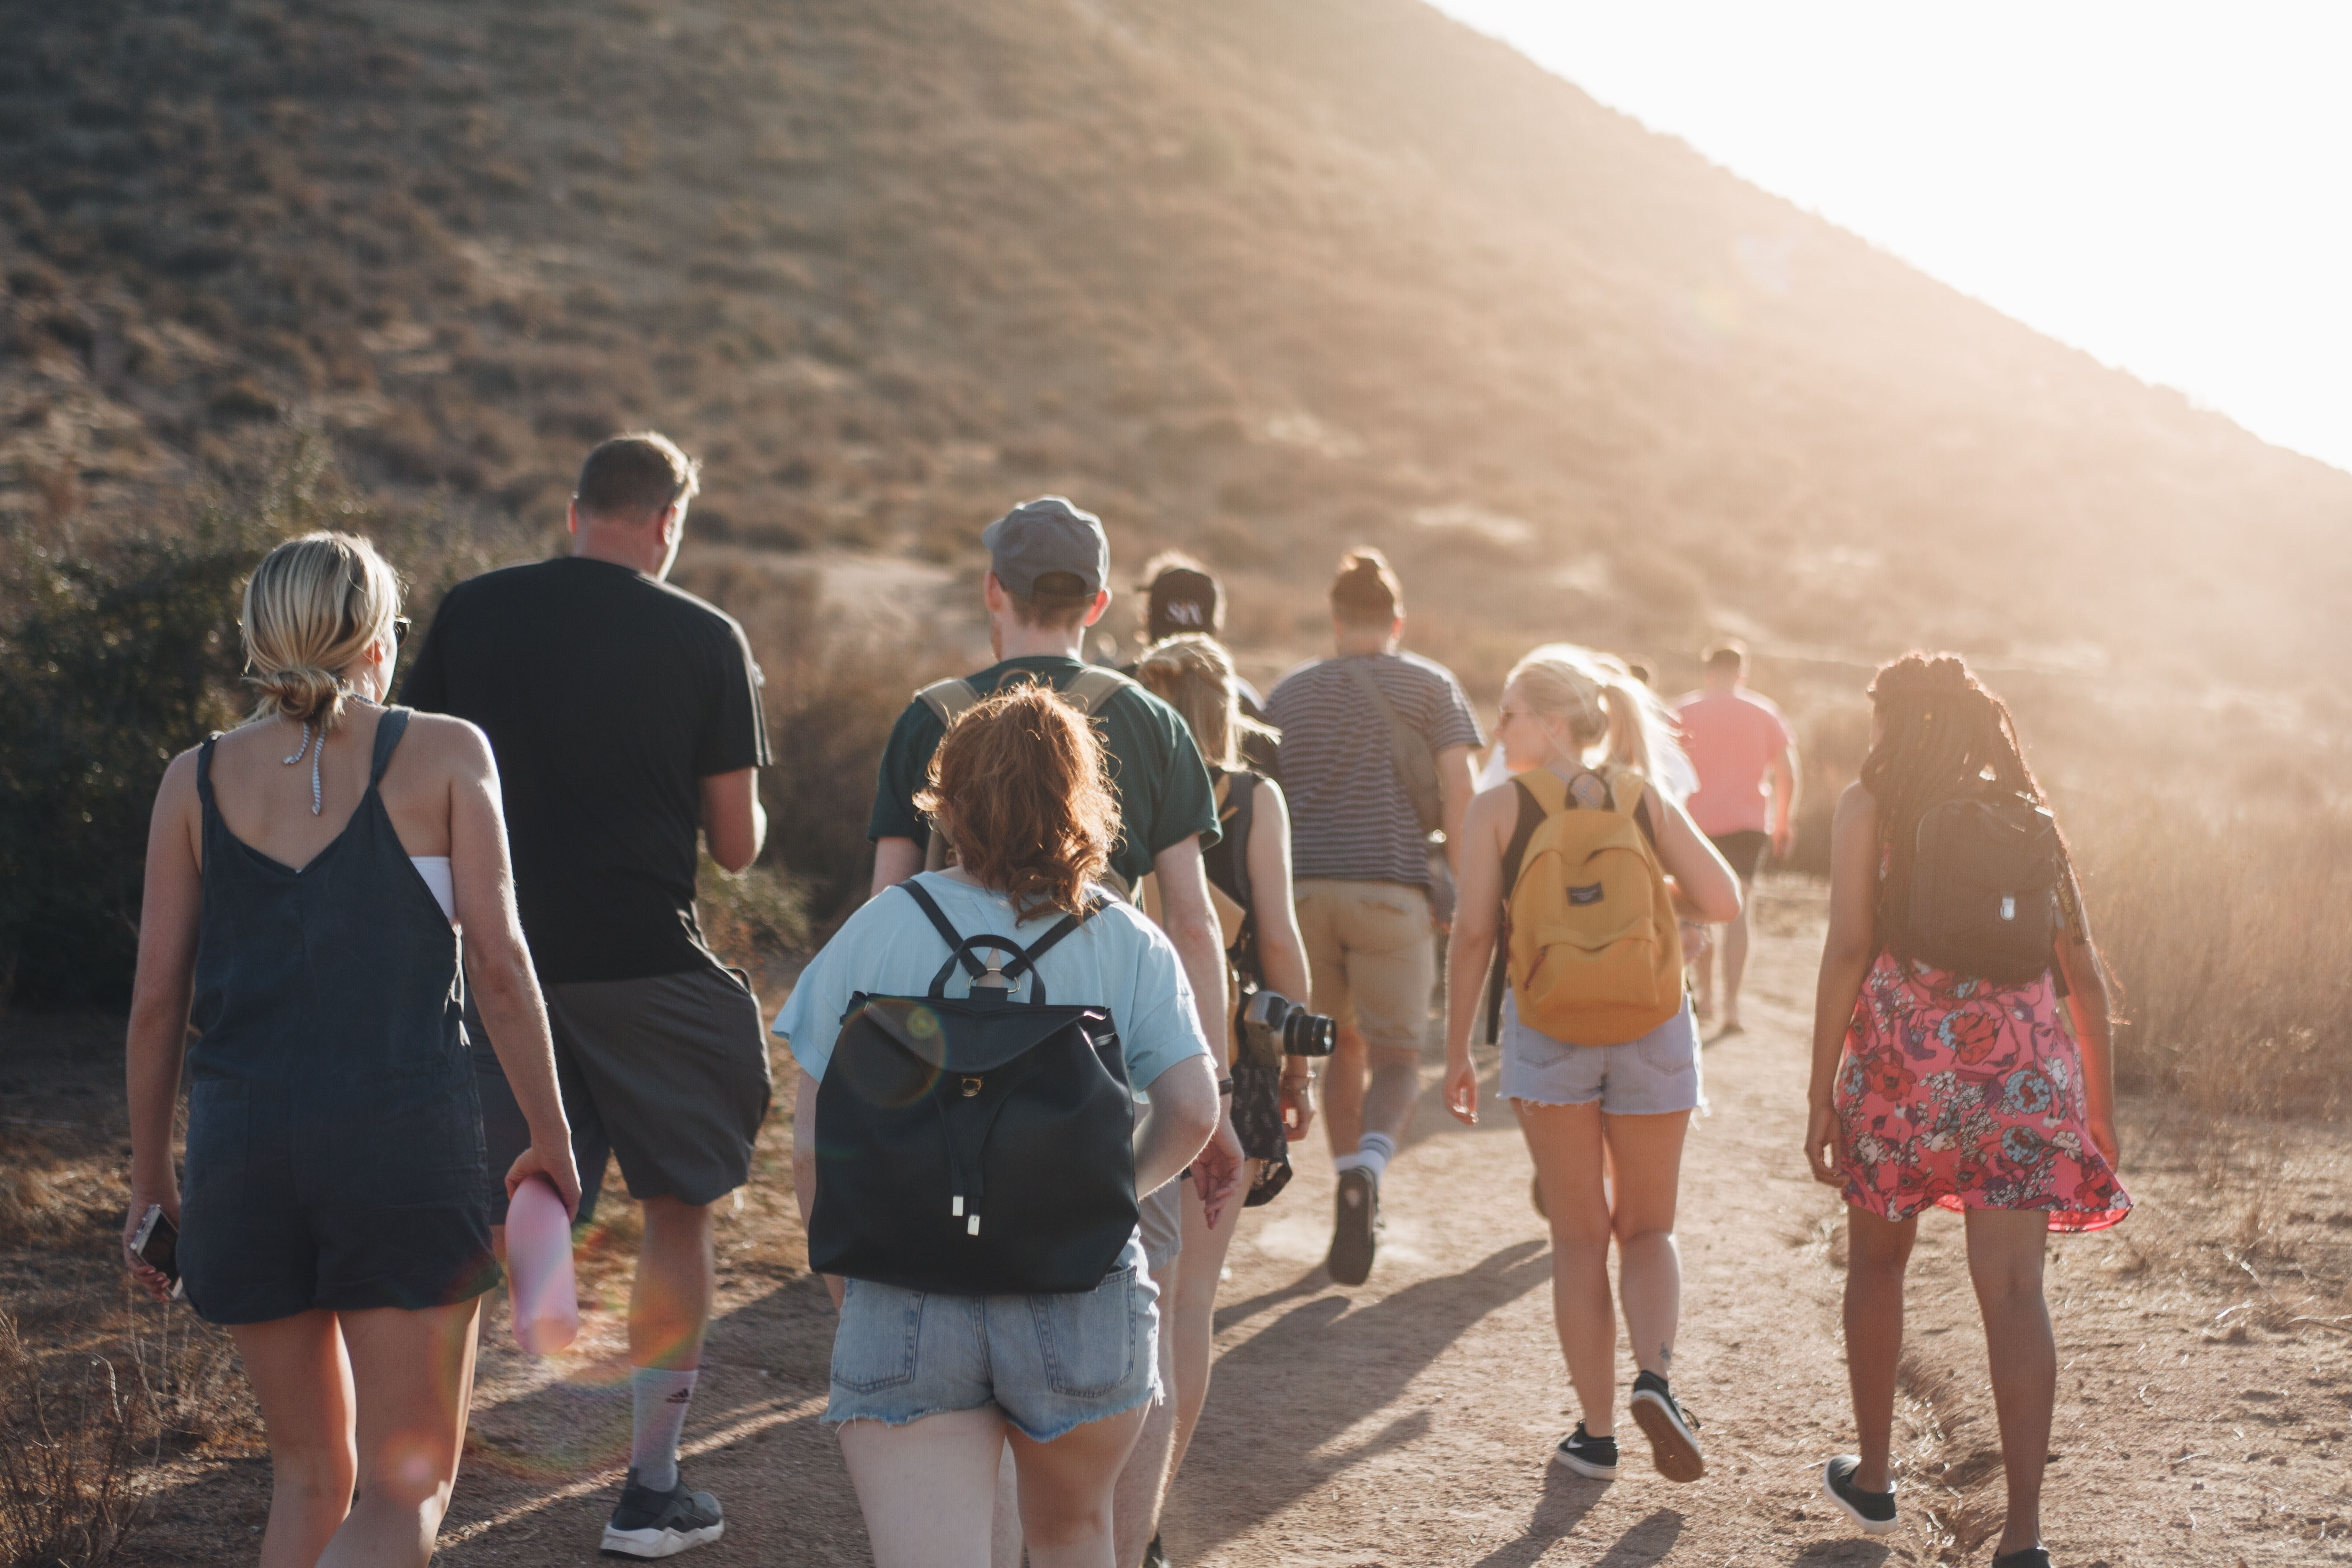
\includegraphics{assets/community/luke-porter-NEqEC7qa9FM-unsplash.jpg}

\hypertarget{title}{%
\chapter{Title}\label{title}}

\hypertarget{title-1}{%
\chapter{Title}\label{title-1}}

\hypertarget{title-2}{%
\chapter{Title}\label{title-2}}

\hypertarget{title-3}{%
\chapter{Title}\label{title-3}}

\hypertarget{title-4}{%
\chapter{Title}\label{title-4}}

\hypertarget{title-5}{%
\chapter{Title}\label{title-5}}

\hypertarget{title-6}{%
\chapter{Title}\label{title-6}}

\hypertarget{title-7}{%
\chapter{Title}\label{title-7}}

\hypertarget{assessment}{%
\chapter*{Assessment}\label{assessment}}
\addcontentsline{toc}{chapter}{Assessment}

The following assignments are opportunities for learners to demonstrate their understanding of the course outcomes. Please confirm assignment details with your instructor, referring to the course syllabus.

Note that Assignment dropboxes are located in Moodle. Also refer to the Course Schedule in Moodle for the specific due dates.

\hypertarget{assignment}{%
\section*{Assignment:}\label{assignment}}
\addcontentsline{toc}{section}{Assignment:}

\begin{assessment}

\end{assessment}

\hypertarget{grading-criteria}{%
\subsection*{Grading Criteria}\label{grading-criteria}}
\addcontentsline{toc}{subsection}{Grading Criteria}

See the following rubric that explains how your assignment will be evaluated. Also available as a \href{assets/assessment/Identity-as-a-Teacher-RUBRIC.pdf}{pdf}

\#\#\#\# APA/WRITING \{-\}

\textbf{Unsatisfactory:} Paper does not model language and conventions used in scholarly literature. Writing is not well-organized. Several errors in grammar or composition. Sources are not cited. APA citations are not appropriately formatted.

\textbf{Developing:} Paper partially models language and conventions used in scholarly literature. Writing is somewhat well organized and includes some errors in grammar or composition. Not all sources cited. APA citations are generally formatted correctly, with several errors.

\textbf{Proficient:} \emph{Paper consistently models language and conventions used in scholarly literature. Writing is well-organized and includes few (if any) errors in grammar or composition. All resources are appropriately cited (including in-text citations and bibliography information). Few (if any) errors in APA citations.}

\textbf{Exemplary:} Paper is an exemplar of language and conventions used in scholarly literature. Writing is well-organized and free of errors in grammar or composition. All resources are appropriately cited. No errors in APA format.

\hypertarget{statement-of-teaching-identity}{%
\subsubsection*{STATEMENT OF TEACHING IDENTITY}\label{statement-of-teaching-identity}}
\addcontentsline{toc}{subsubsection}{STATEMENT OF TEACHING IDENTITY}

\textbf{Unsatisfactory:} Does not provide a statement about identity as a teacher/facilitator

\textbf{Developing:} Provides an unclear statement about identity as a teacher/facilitator.

\textbf{Proficient:} \emph{Provides a clear, concise, and powerful statement about identity as a teacher/facilitator.}

\textbf{Exemplary:} Provides a clear, concise, and powerful statement about identity as a teacher/facilitator. Statement incorporates theory or research from course materials.

\hypertarget{developing-a-cohesive-and-logical-academic-argument}{%
\subsubsection*{DEVELOPING A COHESIVE AND LOGICAL ACADEMIC ARGUMENT}\label{developing-a-cohesive-and-logical-academic-argument}}
\addcontentsline{toc}{subsubsection}{DEVELOPING A COHESIVE AND LOGICAL ACADEMIC ARGUMENT}

\textbf{Unsatisfactory:} Does not make a focused, cohesive, or logical academic argument. Paper is confusing, and is missing an introduction, body, or conclusion. Transitions between sections and ideas are missing.

\textbf{Developing:} Makes an academic argument that is only partially focused, cohesive and logical. Paper is generally organized, but is missing an introduction, body, or conclusion. Transitions between sections and ideas are unclear.

\textbf{Proficient:} \emph{Makes a focused, cohesive, logical academic argument. Paper is effectively organized and includes an introduction, body, and conclusion. Transitions between sections and ideas are clear.}

\textbf{Exemplary:} Makes a focused, cohesive, logical and compelling academic argument. Paper is effectively organized and includes an introduction, body, and conclusion. Transitions between sections and ideas are clear, and build on each other.

\hypertarget{analysis-of-identity-as-a-teacher}{%
\subsubsection*{ANALYSIS OF IDENTITY AS A TEACHER}\label{analysis-of-identity-as-a-teacher}}
\addcontentsline{toc}{subsubsection}{ANALYSIS OF IDENTITY AS A TEACHER}

\textbf{Unsatisfactory:} Does not include three important aspects of identity as a teacher/facilitator. Does not include an analysis.

\textbf{Developing:} Lists but does not discuss three important aspects of identity as a teacher/facilitator. Includes a partial analysis.

\textbf{Proficient:} \emph{Includes a detailed discussion of three important aspects of identity as a teacher/facilitator. Includes thoughtful analysis of each of the three elements.}

\textbf{Exemplary:} Includes a detailed discussion of three important aspects of identity as a teacher/facilitator. Includes a thoughtful analysis, integrating scholarly literature to support analysis and furthering scholarly thinking related to teacher identity.

\hypertarget{scholarly-integration}{%
\subsubsection*{SCHOLARLY INTEGRATION}\label{scholarly-integration}}
\addcontentsline{toc}{subsubsection}{SCHOLARLY INTEGRATION}

\textbf{Unsatisfactory:} Does not integrate references to support claims and assertions made in the paper.

\textbf{Developing:} Integrates references to support some of the claims and assertions made in the paper.

\textbf{Proficient:} \emph{Integrates references to support claims and assertions made in the paper.}

\textbf{Exemplary:} Integrates references to support claims and assertions made in the paper, effectively synthesizing different perspectives and research results from scholarly sources.

\begin{longtable}[]{@{}
  >{\raggedright\arraybackslash}p{(\columnwidth - 8\tabcolsep) * \real{0.2000}}
  >{\raggedright\arraybackslash}p{(\columnwidth - 8\tabcolsep) * \real{0.2000}}
  >{\raggedright\arraybackslash}p{(\columnwidth - 8\tabcolsep) * \real{0.2000}}
  >{\raggedright\arraybackslash}p{(\columnwidth - 8\tabcolsep) * \real{0.2000}}
  >{\raggedright\arraybackslash}p{(\columnwidth - 8\tabcolsep) * \real{0.2000}}@{}}
\toprule()
\begin{minipage}[b]{\linewidth}\raggedright
\textbf{TOTAL}
\end{minipage} & \begin{minipage}[b]{\linewidth}\raggedright
\textbf{0 = 0\% (F)}
\end{minipage} & \begin{minipage}[b]{\linewidth}\raggedright
\textbf{10 = 50\% (C)}
\end{minipage} & \begin{minipage}[b]{\linewidth}\raggedright
\textbf{15 = 75 (B)}
\end{minipage} & \begin{minipage}[b]{\linewidth}\raggedright
\textbf{20 = 100\% (A+)}
\end{minipage} \\
\midrule()
\endhead
\bottomrule()
\end{longtable}

\begin{center}\rule{0.5\linewidth}{0.5pt}\end{center}

\hypertarget{assignment-company-website-analysis}{%
\section*{Assignment: Company Website Analysis}\label{assignment-company-website-analysis}}
\addcontentsline{toc}{section}{Assignment: Company Website Analysis}

\begin{assessment}
Investigate the Human Resources or Faculty Development portion of a
company's website, a higher education institution or adult learning
facility, preferably one with which you are familiar. Focus on the
faculty or employee development part of the website. In this assignment,
you will apply the theory of teaching in/for/with depth by analyzing the
learning culture of an organization.

In a 4-5 page APA formatted paper, analyze the website by responding to
the following questions in your report:

\begin{enumerate}
\def\labelenumi{\arabic{enumi}.}
\tightlist
\item
  What can you infer about the company's learning culture?
\item
  From what is visible on the public website, would you say it is an
  authentic learning community? Why or why not? Discuss whether the
  website reflects aspects of one or more of the learning community
  models explored in previous lessons.
\item
  Do you see evidence that interconnectedness and integrity are valued?
  Explain.
\item
  What traits and skills seem to be valued in employees?
\item
  How does the company develop skills in its employees (e.g., workshops,
  seminars, mentoring)? Are the methods based on the principles of
  andragogy? (see Smith YouTube video). What specific adult learning
  strategies do you see reflected in the development/training
  opportunities for employees?
\end{enumerate}

Your paper should be 4-5 pages and should incorporate references to at
least five scholarly sources you have studied in this course, or other
scholarly sources you have identified.

The paper should include:

\begin{enumerate}
\def\labelenumi{\arabic{enumi}.}
\tightlist
\item
  Introduction
\item
  Analysis (responding to the prompts)
\item
  Conclusion
\item
  Reference List
\end{enumerate}
\end{assessment}

\hypertarget{company-website-analysis-rubric}{%
\subsection*{Company Website Analysis Rubric}\label{company-website-analysis-rubric}}
\addcontentsline{toc}{subsection}{Company Website Analysis Rubric}

See the following rubric that explains how your assignment will be evaluated. Also available as a \href{assets/assessment/Company-Website-Analysis-RUBRIC.pdf}{pdf}

\hypertarget{apa-formatting}{%
\subsubsection*{APA Formatting}\label{apa-formatting}}
\addcontentsline{toc}{subsubsection}{APA Formatting}

\textbf{Unsatisfactory:} Paper does not model language and conventions used in scholarly literature.
Writing is not well-organized. Several errors in grammar or composition. Sources
are not cited. APA citations are not appropriately formatted.

\textbf{Developing:} Paper partially models language and conventions used in scholarly literature.
Writing is somewhat well organized and includes some errors in grammar or
composition. Not all sources cited. APA citations are generally formatted
correctly, with several errors.

\textbf{Proficient:} \emph{Paper consistently models language and conventions used in scholarly
literature. Writing is well-organized and includes few (if any) errors in
grammar or composition. All resources are appropriately cited (including in-text
citations and bibliography information). Few (if any) errors in APA citations.}

\textbf{Exemplary:} Paper is an exemplar of language and conventions used in scholarly literature.
Writing is well-organized and free of errors in grammar or composition. All
resources are appropriately cited. No errors in APA format.

\hypertarget{developing-a-cohesive-and-logical-academic-argument-1}{%
\subsubsection*{DEVELOPING a COHESIVE and LOGICAL ACADEMIC ARGUMENT}\label{developing-a-cohesive-and-logical-academic-argument-1}}
\addcontentsline{toc}{subsubsection}{DEVELOPING a COHESIVE and LOGICAL ACADEMIC ARGUMENT}

\textbf{Unsatisfactory:} Does not make a focused, cohesive, or logical academic argument. Paper is
confusing, and is missing an introduction, body, or conclusion. Transitions
between sections and ideas are missing.

\textbf{Developing:} Makes an academic argument that is only partially focused, cohesive and logical.
Paper is generally organized, but is missing an introduction, body, or
conclusion. Transitions between sections and ideas are unclear.

\textbf{Proficient:} \emph{Makes a focused, cohesive, logical academic argument. Paper is effectively
organized and includes an introduction, body, and conclusion. Transitions
between sections and ideas are clear.}

\textbf{Exemplary:} Makes a focused, cohesive, logical and compelling academic argument. Paper is
effectively organized and includes an introduction, body, and conclusion.
Transitions between sections and ideas are clear and build on each other.

\hypertarget{analysis-of-learning-culture}{%
\subsubsection*{ANALYSIS of LEARNING CULTURE}\label{analysis-of-learning-culture}}
\addcontentsline{toc}{subsubsection}{ANALYSIS of LEARNING CULTURE}

\textbf{Unsatisfactory:} Does not include an analysis of the company learning culture, and no evaluation
of the authenticity of the learning community.

\textbf{Developing:} Includes a partial analysis of the company learning culture, including a limited
evaluation of the authenticity of the learning community.

\textbf{Proficient:} \emph{Includes a detailed analysis of the company learning culture, including an
evaluation of the authenticity of the learning community.}

\textbf{Exemplary:} Includes a detailed analysis of the company learning culture, including an
evaluation of the authenticity of the learning community. Includes a thoughtful
analysis, integrating scholarly literature to support analysis and furthering
scholarly thinking related to teacher identity.

\hypertarget{evaluation-of-interconnectedness-and-integrity}{%
\subsubsection*{EVALUATION of INTERCONNECTEDNESS and INTEGRITY}\label{evaluation-of-interconnectedness-and-integrity}}
\addcontentsline{toc}{subsubsection}{EVALUATION of INTERCONNECTEDNESS and INTEGRITY}

\textbf{Unsatisfactory:} Does not include an evaluation of evidence of interconnectedness and integrity
on the company website. Does not integrate scholarly sources in the evaluation.

\textbf{Developing:} Includes a partial evaluation of evidence of interconnectedness and integrity on
the company website. Evaluation includes only limited reference to scholarly
sources.

\textbf{Proficient:} \emph{Includes a detailed evaluation of evidence of interconnectedness and integrity
on the company website. Evaluation integrates scholarly sources.}

\textbf{Exemplary:} Includes a detailed evaluation of evidence of interconnectedness and integrity
on the company website. Includes recommendations for ways in which to integrate
interconnectedness and integrity into employee development.

\hypertarget{analysis-of-adult-learning-strategies}{%
\subsubsection*{ANALYSIS of ADULT LEARNING STRATEGIES}\label{analysis-of-adult-learning-strategies}}
\addcontentsline{toc}{subsubsection}{ANALYSIS of ADULT LEARNING STRATEGIES}

\textbf{Unsatisfactory:} Does not include a detailed analysis of valued skills and evidence of adult
learning theory in employee development. Does not integrate scholarly sources.

\textbf{Developing:} Includes a partial analysis of valued skills and evidence of adult learning
theory in employee development. Analysis integrates few, if any, scholarly
sources.

\textbf{Proficient:} \emph{Includes a detailed analysis of valued skills and evidence of adult learning
theory in employee development. Analysis integrates scholarly sources.}

\textbf{Exemplary:} Includes a detailed analysis of valued skills and evidence of adult learning
theory in employee development. Includes recommendations for ways in which to
integrate adult learning theory into employee development.

\hypertarget{scholarly-integration-1}{%
\subsubsection*{SCHOLARLY INTEGRATION}\label{scholarly-integration-1}}
\addcontentsline{toc}{subsubsection}{SCHOLARLY INTEGRATION}

\textbf{Unsatisfactory:} Does not integrate scholarly references to support claims and assertions made in
the paper.

\textbf{Developing:} Integrates scholarly references to support some of the claims and assertions
made in the paper.

\textbf{Proficient:} \emph{Integrates scholarly references to support claims and assertions made in the
paper.}

\textbf{Exemplary:} Integrates scholarly references to support claims and assertions made in the
paper, effectively synthesizing different perspectives and research results from
scholarly sources.

\begin{longtable}[]{@{}
  >{\raggedright\arraybackslash}p{(\columnwidth - 8\tabcolsep) * \real{0.2000}}
  >{\raggedright\arraybackslash}p{(\columnwidth - 8\tabcolsep) * \real{0.2000}}
  >{\raggedright\arraybackslash}p{(\columnwidth - 8\tabcolsep) * \real{0.2000}}
  >{\raggedright\arraybackslash}p{(\columnwidth - 8\tabcolsep) * \real{0.2000}}
  >{\raggedright\arraybackslash}p{(\columnwidth - 8\tabcolsep) * \real{0.2000}}@{}}
\toprule()
\begin{minipage}[b]{\linewidth}\raggedright
\textbf{TOTAL}
\end{minipage} & \begin{minipage}[b]{\linewidth}\raggedright
\textbf{0 = 0\% (F)}
\end{minipage} & \begin{minipage}[b]{\linewidth}\raggedright
\textbf{10 = 50\% (C)}
\end{minipage} & \begin{minipage}[b]{\linewidth}\raggedright
\textbf{15 = 75 (B)}
\end{minipage} & \begin{minipage}[b]{\linewidth}\raggedright
\textbf{20 = 100\% (A+)}
\end{minipage} \\
\midrule()
\endhead
\bottomrule()
\end{longtable}

\begin{center}\rule{0.5\linewidth}{0.5pt}\end{center}

\hypertarget{assignment-platform-paper}{%
\section*{Assignment: Platform Paper}\label{assignment-platform-paper}}
\addcontentsline{toc}{section}{Assignment: Platform Paper}

\begin{assessment}
For this assignment, you will write a contextualized Platform Paper in
which you discuss your ideal learning community and your role as
teacher/leader of that learning community. Select a context for your
paper (i.e.~facilitating in a FAR Centre in a specific country, teaching
adult learners, facilitating employee development workshops, etc.). Your
paper should be written and referenced in APA format and include
references to a minimum of 10 scholarly sources (this can include
literature you read in this course). You will write a draft of the
Platform Paper in Unit 8 and post for Peer Review. In Unit 9, you will
provide feedback to another learner on their paper. You will make
revisions based on the Peer Review and, in Unit 10, you will submit the
final Platform Paper. Peer reviewers will be assigned in advance.

\hypertarget{paper-outline}{%
\subsubsection{Paper Outline}\label{paper-outline}}

This paper will be 12-15 pages long, and should include: 1. Introduction
(1-2 pages) 2. Section 1: Ideal Learning Environment (5-7 pages) 3.
Section 2: Your Role as Teacher and Leader (5-7 pages) 4. Conclusion
(1-2 pages)

\hypertarget{paper-guidelines}{%
\subsubsection{Paper Guidelines}\label{paper-guidelines}}

\begin{itemize}
\tightlist
\item
  \textbf{Introduction}: Introduce the two sections in your paper,
  providing a brief description of the key points you will make in each
  section.
\item
  \textbf{Section 1}: In section one, you will describe your ideal
  education learning environment. This section should demonstrate your
  learning about authentic learning communities, incorporating scholarly
  sources and your own analysis to depict your ideal learning
  environment. Incorporate a discussion of the learning community
  environment, learning experiences, student learning outcomes, and
  personal beliefs about teaching and learning.
\item
  \textbf{Section 2}: In this section, describe your role as a teacher
  or leader within an authentic learning community. Incorporating
  scholarly literature, analyze your role as a facilitator/leader in
  planning learning experiences, facilitating student learning, and
  assessing student learning. Describe the actions, practices, and
  strategies you will engage in to achieve your vision of the learning
  community you described in section one.
\item
  \textbf{Conclusion}: Summarize the key points you made in each
  section.
\item
  \textbf{References}: Include a reference list with references to at
  least 10 scholarly sources.
\end{itemize}
\end{assessment}

\hypertarget{platform-paper-rubric}{%
\subsection*{Platform Paper Rubric}\label{platform-paper-rubric}}
\addcontentsline{toc}{subsection}{Platform Paper Rubric}

See the following rubric that explains how your assignment will be evaluated. Also available as a \href{assets/assessment/Platform-Paper-RUBRIC.pdf}{pdf}

\hypertarget{apawriting}{%
\subsubsection*{APA/WRITING}\label{apawriting}}
\addcontentsline{toc}{subsubsection}{APA/WRITING}

\textbf{Unsatisfactory:} Paper does not model language and conventions used in scholarly literature. Writing is not well-organized. Several errors in grammar or composition. Sources are not cited. APA citations are not appropriately formatted.

\textbf{Developing:} Paper partially models language and conventions used in scholarly literature. Writing is somewhat well organized and includes some errors in grammar or composition. Not all sources cited. APA citations are generally formatted correctly, with several errors.

\textbf{Proficient:} \emph{Paper consistently models language and conventions used in scholarly literature. Writing is well-organized and includes few (if any) errors in grammar or composition. All resources are appropriately cited (including in-text citations and bibliography information). Few (if any) errors in APA citations.}

\textbf{Exemplary:} Paper is an exemplar of language and conventions used in scholarly literature. Writing is well-organized and free of errors in grammar or composition. All resources are appropriately cited. No errors in APA format.

\hypertarget{developing-a-cohesive-and-logical-academic-argument-2}{%
\subsubsection*{DEVELOPING a COHESIVE and LOGICAL ACADEMIC ARGUMENT}\label{developing-a-cohesive-and-logical-academic-argument-2}}
\addcontentsline{toc}{subsubsection}{DEVELOPING a COHESIVE and LOGICAL ACADEMIC ARGUMENT}

\textbf{Unsatisfactory:} Does not make a focused, cohesive, or logical academic argument. Paper is confusing, and is missing an introduction, body, or conclusion. Transitions between sections and ideas are missing.

\textbf{Developing:} Makes an academic argument that is only partially focused, cohesive and logical. Paper is generally organized, but is missing an introduction, body, or conclusion. Transitions between sections and ideas are unclear.

\textbf{Proficient:} \emph{Makes a focused, cohesive, logical academic argument. Paper is effectively organized and includes an introduction, body, and conclusion. Transitions between sections and ideas are clear.}

\textbf{Exemplary:} Makes a focused, cohesive, logical and compelling academic argument. Paper is effectively organized and includes an introduction, body, and conclusion. Transitions between sections and ideas are clear, and build on each other.

\hypertarget{ideal-learning-environment}{%
\subsubsection*{IDEAL LEARNING ENVIRONMENT}\label{ideal-learning-environment}}
\addcontentsline{toc}{subsubsection}{IDEAL LEARNING ENVIRONMENT}

\textbf{Unsatisfactory:} Does not include a description of your ideal learning environment. Does not reference scholarly sources. Does note analyze key elements of an authentic learning community. Does not mention or describe the learning community environment, student learning outcomes, learning outcomes and personal beliefs about teaching and learning.

\textbf{Developing:} Includes a partial description of your ideal learning environment, referencing few scholarly sources and including a partial analysis of key elements of an authentic learning community. Mentions some elements, but does not fully describe the learning community environment, student learning outcomes, learning outcomes and personal beliefs about teaching and learning.

\textbf{Proficient:} \emph{Includes a detailed description of your ideal learning environment, referencing scholarly sources and analyzing key elements of an authentic learning community. Describes the learning community environment, student learning outcomes, learning outcomes and personal beliefs about teaching and learning.}

\textbf{Exemplary:} Includes a detailed description of your ideal learning environment, referencing scholarly sources and analyzing key elements of authentic learning communities. Provides a rationale for key elements of the learning community environment, student learning outcomes, learning outcomes and personal beliefs about teaching and learning. Advances scholarly thinking about authentic learning communities.

\hypertarget{your-role-as-teacher-and-leaders}{%
\subsubsection*{YOUR ROLE AS TEACHER AND LEADERS}\label{your-role-as-teacher-and-leaders}}
\addcontentsline{toc}{subsubsection}{YOUR ROLE AS TEACHER AND LEADERS}

\textbf{Unsatisfactory:} Does not include a description of your role as a teacher or leader within an authentic learning community, incorporating scholarly literature. Does not include an analysis of your role as a facilitator/leader in planning learning experiences, facilitating student learning, and assessing student learning. Does not include a description of the actions, practices, and strategies you will engage in to achieve your vision of the learning community you described in section one.

\textbf{Developing:} Includes a partial description of your role as a teacher or leader within an authentic learning community, incorporating scholarly literature. Describes but does not analyze your role as a facilitator/leader in planning learning experiences, facilitating student learning, and assessing student learning. Lists but does not describe the actions, practices, and strategies you will engage in to achieve your vision of the learning community you described in section one.

\textbf{Proficient:} \emph{Includes a detailed description of your role as a teacher or leader within an authentic learning community, incorporating scholarly literature. Includes a detailed analysis of your role as a facilitator/leader in planning learning experiences, facilitating student learning, and assessing student learning. Includes a detailed description of the actions, practices, and strategies you will engage in to achieve your vision of the learning community you described in section one.}

\textbf{Exemplary:} Includes a detailed analysis of your role as a teacher or leader within an authentic learning community, incorporating scholarly literature. Includes a detailed analysis of your role as a facilitator/leader in planning learning experiences, facilitating student learning, and assessing student learning. Includes a detailed description of the actions, practices, and strategies you will engage in to achieve your vision of the learning community you described in section one. Synthesizes scholarly thinking about the role of the teacher/leader.

\hypertarget{scholarly-integration-2}{%
\subsubsection*{SCHOLARLY INTEGRATION}\label{scholarly-integration-2}}
\addcontentsline{toc}{subsubsection}{SCHOLARLY INTEGRATION}

\textbf{Unsatisfactory:} Does not integrate many references to support the arguments made in the paper.

\textbf{Developing:} Integrates fewer than 10 scholarly sources to support arguments made in the paper.

\textbf{Proficient:} \emph{Integrates a minimum of 10 scholarly sources to support arguments made in each section of the paper.}

\textbf{Exemplary:} Integrates a minimum of 10 references to support the arguments made in each section, including several scholarly sources not included in course materials.

\begin{longtable}[]{@{}
  >{\raggedright\arraybackslash}p{(\columnwidth - 8\tabcolsep) * \real{0.2000}}
  >{\raggedright\arraybackslash}p{(\columnwidth - 8\tabcolsep) * \real{0.2000}}
  >{\raggedright\arraybackslash}p{(\columnwidth - 8\tabcolsep) * \real{0.2000}}
  >{\raggedright\arraybackslash}p{(\columnwidth - 8\tabcolsep) * \real{0.2000}}
  >{\raggedright\arraybackslash}p{(\columnwidth - 8\tabcolsep) * \real{0.2000}}@{}}
\toprule()
\begin{minipage}[b]{\linewidth}\raggedright
\textbf{TOTAL}
\end{minipage} & \begin{minipage}[b]{\linewidth}\raggedright
\textbf{0 = 0\% (F)}
\end{minipage} & \begin{minipage}[b]{\linewidth}\raggedright
\textbf{10 = 50\% (C)}
\end{minipage} & \begin{minipage}[b]{\linewidth}\raggedright
\textbf{15 = 75 (B)}
\end{minipage} & \begin{minipage}[b]{\linewidth}\raggedright
\textbf{20 = 100\% (A+)}
\end{minipage} \\
\midrule()
\endhead
\bottomrule()
\end{longtable}

\hypertarget{references}{%
\chapter*{References}\label{references}}
\addcontentsline{toc}{chapter}{References}

The following are key references used in this course. \textbf{\emph{Check with your course syllabus for required readings.}}

  \bibliography{book.bib}

\end{document}
